\subsection{扩张}

定义 1. 设 F 和 G 是两个群。G 被 F 的扩张是一个三元组 \(\mathcal{E} = (\mathrm{E}, i, p)\) ，其中 E 是一个群， \(i\) 是 F 到 E 内的单射同态， \(p\) 是 E 到 G 上的满射同态，使得 \(\operatorname{Im}(i) = \operatorname{Ker}(p)\) 。同态 \(s: \mathrm{G} \to \mathrm{E}\) （相应地， \(r: \mathrm{E} \to \mathrm{F}\) ），若满足 \(p \circ s = \operatorname{Id}_{\mathbf{G}}\) （相应地， \(r \circ i = \operatorname{Id}_{\mathbf{F}}\) ），则称为扩张 \(\mathcal{E}\) 的截面（相应地，收缩）。

扩张 \(\mathcal{E} = (\mathrm{E}, i, p)\) （ \(\mathbf{G}\) 被 \(\mathbf{F}\) 的扩张）常用图表 \(\mathcal{E}: \mathrm{F} \xrightarrow{i} \mathrm{E} \xrightarrow{p} \mathrm{G}\) 表示，其中 \(i\) 和 \(p\) 在不会引起混淆时有时省略。有时也简单地说群 \(\mathbf{E}\) 是 \(\mathbf{G}\) 被 \(\mathbf{F}\) 的扩张。

群 E 是 G 被 F 的扩张，当且仅当它包含一个同构于 F 的正规子群 \(F'\) ，使得商群 \(E/F'\) 同构于 G。

一个扩张 \(\mathcal{E}\colon\mathrm{F}\xrightarrow{i}\mathrm{E}\xrightarrow{p}\mathrm{G}\) 称为中心扩张，如果像 \(i(\mathrm{F})\) 包含在 E 的中心内；这仅当 F 是交换群时才可能。

设 \(\mathcal{E}:\mathrm{F}\xrightarrow{i}\mathrm{E}\xrightarrow{p}\mathrm{G}\) 和 \(\mathcal{E}':\mathrm{F}\xrightarrow{i'}\mathrm{E}'\xrightarrow{p'}\mathrm{G}\) 是 G 被 F 的两个扩张。\(\mathcal{E}\) 到 \(\mathcal{E}'\) 的态射是一个同态 \(u:\mathrm{E}\to\mathrm{E}'\) ，满足 \(p'\circ u=p\) 与 \(u\circ i=i'\) ，或者换句话说，使得下图交换：

\pandocbounded{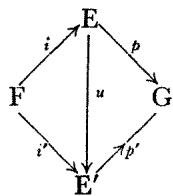
\includegraphics[keepaspectratio]{images/part001_e41623d9.jpg}}

命题 1. 设 \(\mathcal{E}: F \xrightarrow{i} E \xrightarrow{p} G\) 和 \(\mathcal{E}': F \xrightarrow{i'} E' \xrightarrow{p'} G\) 是 \(G\) 被 \(F\) 的扩张。若 \(u: E \to E'\) 是 \(\mathcal{E}\) 到 \(\mathcal{E}'\) 的态射，则 \(u\) 是 \(E\) 到 \(E'\) 上的同构，且 \(u^{-1}\) 是 \(\mathcal{E}'\) 到 \(\mathcal{E}\) 的态射。

设 \(x \in E\) 满足 \(u(x) = e\) 。则 \(p(x) = p'(u(x)) = e\) ，因此 \(x \in i(F)\) 。设 \(y \in F\) 满足 \(x = i(y)\) ；则 \(i'(y) = u(i(y)) = e\) 。由于 \(i'\) 是单射，有 \(y = e\) 与 \(x = e\) 。因此 \(u\) 是单射。根据 §4 第 6 号命题 7 的推论 1 ， \(u\) 是满射，因为 \(u(i(F)) = i'(F)\) 。最后一个断言是显然的。

换句话说，扩张 \(\mathcal{E}\) 与 \(\mathcal{E}'\) 同构，当且仅当存在 \(\mathcal{E}\) 到 \(\mathcal{E}'\) 的态射。

设 \(\mathbf{F}\) 和 \(\mathbf{G}\) 是两个群，记 \(\mathbf{E}_0 = \mathbf{F} \times \mathbf{G}\) ；令 \(i: \mathbf{F} \to \mathbf{E}_0\) 为典范单射， \(p: \mathbf{E}_0 \to \mathbf{G}\) 为典范投影。\(\mathbf{G}\) 被 \(\mathbf{F}\) 的扩张中，凡同构于扩张 \(\mathcal{E}_0: \mathbf{F} \xrightarrow{i} \mathbf{E}_0 \xrightarrow{p} \mathbf{G}\) 者，都称为平凡扩张。

命题 2. 设 \(\mathcal{E}:\mathrm{F}\xrightarrow{i}\mathrm{E}\xrightarrow{p}\mathrm{G}\) 是 \(\mathrm{G}\) 被 \(\mathrm{F}\) 的一个扩张。下列条件等价：

\begin{enumerate}
\def\labelenumi{(\roman{enumi})}
\item
  \(\mathcal{E}\) 是一个平凡扩张；
\item
  \(\mathcal{E}\) 有一个收缩 \(r\) ；
\item
  \(\mathcal{E}\) 有一个截面 \(s\) ，使得 \(s(\mathbf{G})\) 包含于 \(i(\mathbf{F})\) 的中心化子中；
\end{enumerate}

显然 (i) 蕴含 (ii) 与 (iii)。若 (ii) 成立，则映射 \((r, p): \mathbf{E} \to \mathbf{F} \times \mathbf{G}\) 是 \(\mathcal{E}\) 到 \(\mathcal{E}_0\) 的态射，由此得 (i)。若 (iii) 成立，则从 \(\mathbf{F} \times \mathbf{G}\) 到 \(\mathbf{E}\) 的、对应于 \((i, s)\) 的同态（ \(\S 4\) ，第 9 号，命题 12）是 \(\mathcal{E}_0\) 到 \(\mathcal{E}\) 的态射，由此得 (i)。

可能有这样的情形：扩张 \(\mathcal{E}:\mathbf{F}\to\mathbf{E}\to\mathbf{G}\) 并不平凡，而群 \(\mathbf{E}\) 却同构于 \(\mathbf{F}\times\mathbf{G}\) （习题 6）。

定义 2. 设 F 和 G 是两个群， \(\tau\) 是 G 到 F 的自同构群的一个同态。记 \(\tau(g)(f) = {}^g f\) （对 \(g \in G\) 与 \(f \in F\) ）。集合 \(\mathbf{F} \times \mathbf{G}\) 赋以合成律

\[
((f, g), (f ^ {\prime}, g ^ {\prime})) \mapsto (f, g) \cdot_ {\tau} (f ^ {\prime}, g ^ {\prime}) = (f. ^ {g} f ^ {\prime}, g g ^ {\prime})\tag{1}
\]

称为 G 与 F 关于 \(\tau\) 的外半直积。

G 与 F 关于 \(\tau\) 的外半直积记作 \(F \times_{\tau} G\) 。

命题 3. 外半直积 \(\mathbf{F} \times_{\tau} \mathbf{G}\) 是一个群。映射 \(i: \mathbf{F} \to \mathbf{F} \times_{\tau} \mathbf{G}\) 由 \(i(f) = (f, e)\) 定义，映射 \(p: \mathbf{F} \times_{\tau} \mathbf{G} \to \mathbf{G}\) 由 \(p(f, g) = g\) 定义，映射 \(s: \mathbf{G} \to \mathbf{F} \times_{\tau} \mathbf{G}\) 由 \(s(g) = (e, g)\) 定义，它们都是群同态。三元组 \((\mathbf{F} \times_{\tau} \mathbf{G}, i, p)\) 是 \(\mathbf{G}\) 被 \(\mathbf{F}\) 的一个扩张，而 \(s\) 是该扩张的一个截面。

我们有：

\[
\begin{array}{r l} ((f, g) \cdot_ {\tau} (f ^ {\prime}, g ^ {\prime})) \cdot_ {\tau} (f ^ {\prime \prime}, g ^ {\prime \prime}) & = (f. ^ {g} f ^ {\prime}, g g ^ {\prime}) \cdot_ {\tau} (f ^ {\prime \prime}, g ^ {\prime \prime}) \\ & = (f. ^ {g} f ^ {\prime}. ^ {g g ^ {\prime}} f ^ {\prime \prime}, g g ^ {\prime} g ^ {\prime \prime}); \\ (f, g) \cdot_ {\tau} ((f ^ {\prime}, g ^ {\prime}) \cdot_ {\tau} (f ^ {\prime \prime}, g ^ {\prime \prime})) & = (f, g) \cdot_ {\tau} (f ^ {\prime}. ^ {g ^ {\prime}} f ^ {\prime \prime}, g ^ {\prime} g ^ {\prime \prime}) \\ & = (f. ^ {g} (f ^ {\prime}. ^ {g ^ {\prime}} f ^ {\prime \prime}), g g ^ {\prime} g ^ {\prime \prime}). \end{array}
\]

现在， \({}^{g}(f'.{}^{g'}f'') = {}^{g}f'.{}^{gg'}f''\) ，这表明由 (1) 定义的合成律是结合的。元素 \((e, e)\) 是该律下的单位元。元素 \((f, g)\) 以 \((^{g^{-1}}f^{-1}, g^{-1})\) 为逆元。因此 \(F \times_{\tau} G\) 上的合成律是群律。其余断言是显然的。

采用命题 3 的记号，用 \(E_{\tau}\) 表示扩张

\[
\mathrm{F} \xrightarrow {i} \mathrm{F} \times_ {\tau} \mathrm{G} \xrightarrow {p} \mathrm{G}.
\]

设 \(\mathcal{E}'\colon F\stackrel{i'}{\to}E'\stackrel{p'}{\to}G\) 是 \(G\) 被 \(F\) 的扩张， \(s'\colon G\to E'\) 是 \(\mathcal{E}'\) 的一个截面。我们定义一个运算 \(\tau\) （ \(G\) 在群 \(F\) 上的运算）如下：

\[
i ^ {\prime} (\tau (g, f)) = s ^ {\prime} (g) i ^ {\prime} (f) s ^ {\prime} (g) ^ {- 1} = \operatorname{Int} (s ^ {\prime} (g)) (i ^ {\prime} (f)).\tag{2}
\]

命题 4. 采用上述记号，存在唯一的同构 \(u\) ，它把 \(\mathcal{E}_{\tau}\) 映到 \(\mathcal{E}'\) 上，使得 \(u \circ s = s'\) 。

\((f, g) = (f, e) \cdot_ {\tau} (e, g) = i(f).s(g)\) 。因此，如果 u 是该问题的一个解，则必然有 \(u(f,g)=i'(f).s'(g)\) ，从而 u 的唯一性成立。我们证明存在性。我们记 \(u(f,g)=i'(f).s'(g)\) 。则

\[
\begin{array}{r l} u (f, g) \cdot u (f ^ {\prime}, g ^ {\prime}) & = i ^ {\prime} (f) s ^ {\prime} (g) i ^ {\prime} (f ^ {\prime}) s ^ {\prime} (g ^ {\prime}) \\ & = i ^ {\prime} (f) (s ^ {\prime} (g) i ^ {\prime} (f ^ {\prime}) s ^ {\prime} (g) ^ {- 1}) s ^ {\prime} (g) s ^ {\prime} (g ^ {\prime}) \\ & = i ^ {\prime} (f) i ^ {\prime} (\tau (g, f ^ {\prime})) \cdot s ^ {\prime} (g) s ^ {\prime} (g ^ {\prime}) \\ & = i ^ {\prime} (f \cdot \tau (g, f ^ {\prime})) \cdot s ^ {\prime} (g g ^ {\prime}) \\ & = u ((f, g) \cdot_ {\tau} (f ^ {\prime}, g ^ {\prime})). \end{array}
\]

因此， \(u\) 是 \(\mathbf{F} \times_{\tau} \mathbf{G}\) 到 \(\mathbf{E}'\) 内的同态。显然 \(u \circ i = i'\) , \(p' \circ u = p\) 且 \(u \circ s = s'\) 。

注记。由公式 (2) 定义的运算 \(\tau\) 依赖于扩张 \(\mathcal{E}'\) 和截面 \(s'\) 。当 F 交换时，运算 \(\tau\) 不依赖于 \(s'\) 。因为此时 \(\operatorname{Int}(s'(g)) \mid i'(F)\) 仅依赖于 \(s'(g)\) 模 \(i'(F)\) 的陪集。

更一般地，设 \(\mathcal{E}:\mathrm{F}\to \mathrm{E}\to \mathrm{G}\) 是 \(\mathbf{G}\) 被交换群 \(\mathbf{F}\) 的一个扩张（并不假定 \(\mathcal{E}\) 有截面）。群 \(\mathbf{E}\) 经内自同构作用在 \(\mathbf{F}\) 上，该作用在 \(\mathbf{F}\) 的像上平凡，从而定义了 \(\mathbf{G}\) 在 \(\mathbf{F}\) 上的一个作用。若 \(\mathcal{E}\) 有截面，则此作用就是由公式 (2) 定义的作用。

推论. 设 G 是一个群，H 和 K 是 G 的两个子群，使得 H 正规， \(\mathbf{H} \cap \mathbf{K} = \{e\}\) 且 \(\mathbf{H} \cdot \mathbf{K} = \mathbf{G}\) 。设 \(\tau\) 为 \(\mathbf{K}\) 在 \(\mathbf{H}\) 上的、经 \(\mathbf{G}\) 的内自同构定义的作用。映射 \((h, k) \mapsto hk\) 是 \(\mathbf{H} \times_{\tau} \mathbf{K}\) 到 \(\mathbf{G}\) 上的同构。

在此推论的假设下，称 G 为 K 被 H 的半直积。

例子。(1) 设 G 为一个群，E 为一个齐次主 G-集；用 \(\Gamma\) 表示 G 的自同构群。设 A 为 E 的具有下述性质的置换 f 所成的集合：

存在 \(\gamma \in \Gamma\) ，使得 \(f\) 是一个 \(\gamma\) -态射，从 \(\mathbf{E}\) 到 \(\mathbf{E}\) （即 \(f(gb) = \gamma(g)f(b)\) ，对 \(b \in \mathbf{E}\) 与 \(g \in \mathbf{G}\) ）。

上述公式 \(f(gb) = \gamma(g)f(b)\) 表明，若 \(f \in A\) ，则存在唯一的 \(\gamma \in \Gamma\) 使 \(f\) 为 \(\gamma\) -态射，我们把它记作 \(p(f)\) 。

设 \(f, f'\) 是 A 中的元素， \(\gamma = p(f), \gamma' = p(f')\) 。那么，对所有 \(b \in E\) 与所有 \(g \in G\) ，

\[
(f ^ {\prime} \circ f) (g b) = f ^ {\prime} (\gamma (g) f (b)) = \gamma^ {\prime} (\gamma (g)) f ^ {\prime} (f (b))
\]

这证明了 \(f' \circ f \in \mathbf{A}\) 且 \(p(f' \circ f) = p(f')p(f)\) 。另一方面， \(f(\gamma^{-1}(g)f^{-1}(b)) = gb\) ，因此 \(f^{-1}(gb) = \gamma^{-1}(g)f^{-1}(b)\) ，从而 \(f^{-1} \in \mathbf{A}\) 。于是 \(\mathbf{A}\) 是 \(\mathfrak{S}_{\mathbf{E}}\) 的子群， \(p\) 是 \(\mathbf{A}\) 到 \(\Gamma\) 的同态。\(p\) 的核是集合 \(\operatorname{Aut}_{\mathbf{G}}(\mathbf{E})\) ，即 \(\mathbf{G}\) -集 \(\mathbf{E}\) 的自同构组成的集合。

我们取定 \(a \in \mathbf{E}\) 。我们在 §5 第 6 号中定义过一个同构 \(\psi_a\) ，它把 \(\mathbf{G}^0\) 映到 \(\operatorname{Aut}_{\mathbf{G}}(\mathbf{E})\) 上，使得 \(\psi_a(x)(ga) = gxa\) ，其中 \(g, x\) 取遍 \(\mathbf{G}\) 。另一方面，对 \(\gamma \in \Gamma\) ，令 \(s_a(\gamma)\) 为 \(\mathbf{E}\) 的由 \(s_a(\gamma)(ga) = \gamma(g)a\) （对所有 \(g \in \mathbf{G}\) ）定义的置换；立即可验证 \(s_a\) 是 \(\Gamma\) 到 \(\mathbf{A}\) 的同态，且满足 \(p \circ s_a = \operatorname{Id}_{\Gamma}\) 。于是 \(\mathbf{G}^0 \xrightarrow{\psi_a} \mathbf{A} \xrightarrow{p} \Gamma\) 是 \(\Gamma\) 被 \(\mathbf{G}^0\) 的一个扩张，而 \(s_a\) 是该扩张的一个截面。这个扩张与这个截面定义了 \(\Gamma\) 在 \(\mathbf{G}^0\) 上的一个作用： \(s_a(\Gamma)\) 经内自同构作用在 \(\psi_a(\mathbf{G}^0)\) 上；我们把这个作用写成指数记法。我们证明这个作用是自然作用（§3，第 1 号，例 3）：对 \(x, g\) 属于 \(\mathbf{G}\) 以及 \(\gamma \in \Gamma\) ，

\[
\begin{array}{r l} (\psi_ {a} (^ {\gamma} x)) (g a) & = (s _ {a} (\gamma) \circ \psi_ {a} (x) \circ s _ {a} (\gamma) ^ {- 1}) (g a) \\ & = (s _ {a} (\gamma) \circ \psi_ {a} (x)) (\gamma^ {- 1} (g) a) = s _ {a} (\gamma) (\gamma^ {- 1} (g) x a) \\ & = g \gamma (x) a = \psi_ {a} (\gamma (x)) g a \end{array}
\]

，因此 \({}^{\gamma}x = \gamma(x)\) 。

于是命题 4 表明，A 同构于 \(\Gamma = \operatorname{Aut}(\mathbf{G})\) 被 \(\mathbf{G}^0\) 的半直积（在 \(\operatorname{Aut}(\mathbf{G})\) 对 \(\mathbf{G}^0\) 的自然作用下）。注意，我们所构造的同构一般依赖于元素 \(a \in \mathbf{E}\) 的选取。

\begin{enumerate}
\def\labelenumi{(\arabic{enumi})}
\setcounter{enumi}{1}
\tightlist
\item
  *设 A 为交换环。上三角群 T(n, A) 是对角子群 D(n, A) 被上严格三角群 T1(n, A) 的半直积。*
\end{enumerate}

